\chapter{Hormonale regeling van de voortplanting}\label{ch:g11:hormones-and-reproduction}

Een vrouw houdt een schema bij: elke ochtend haar temperatuur, met een
kleine stijging rond het midden van elke maand; een bloeding om de
achtentwintig dagen of daaromtrent. Een laboratorium dat dagelijks vier
\omterm{def:g11:hormones-and-reproduction:hormone}{hormonen} in haar bloed meet, zou vier krommen tekenen die maand na maand
in een vaste volgorde stijgen en dalen, waarbij elke piek de volgende
veroorzaakt. Het schema van een man zou dezelfde \omterm{def:g11:hormones-and-reproduction:hormone}{hormonen} dag na dag op
vrijwel constante niveaus tonen. De organen verschillen; het regelsysteem
--- een centrum in de hersenen, een klier daaronder, de geslachtsklier, en
boodschappen die het bloed in beide richtingen vervoert --- is hetzelfde.
Dit hoofdstuk leest de schema's, en laat zien hoe het begrip ervan het
mogelijk maakte een zwangerschap te voorkomen, of er juist een te
verkrijgen.

\section{Hormonen en hun terugkoppelingen}

\begin{definition}[Hormoon, terugkoppeling]\label{def:g11:hormones-and-reproduction:hormone}
Een \emph{hormoon}\index{hormoon} is een molecuul dat door een klier aan
het bloed wordt afgegeven en dat op afstand inwerkt op de \omterm{def:g10:cells-common-unit:cell}{cellen} die er
een \emph{receptor} voor dragen. Een hormoonstelsel wordt geregeld door
\emph{terugkoppeling}\index{terugkoppeling}: het hormoon dat aan het eind
van een keten wordt gemaakt, werkt terug op de klieren aan het begin
ervan. \emph{Negatieve terugkoppeling} --- het product vermindert het
bevel --- houdt een niveau constant; \emph{positieve terugkoppeling} ---
het product versterkt het bevel --- brengt een uitschieter voort.
\end{definition}

\begin{proposition}[De gemeenschappelijke keten]\label{prop:g11:hormones-and-reproduction:chain}
Bij beide geslachten stuurt dezelfde keten van drie lagen de
geslachtsklieren aan. Een centrum in de hersenen, de
\emph{hypothalamus}, geeft in stoten een vrijzettend \omterm{def:g11:hormones-and-reproduction:hormone}{hormoon}, GnRH, af
aan de kleine vaten die naar de \emph{hypofyse} daar vlak onder leiden;
de hypofyse antwoordt door twee \omterm{def:g11:hormones-and-reproduction:hormone}{hormonen} aan het algemene bloed af te
geven, \emph{LH} en \emph{FSH}; die werken op de geslachtsklieren, die
zowel gameten als geslachtshormonen voortbrengen --- testosteron in de
teelbal, oestrogenen en progesteron in de eierstok. De
geslachtshormonen werken op het lichaam, en werken terug op de
hypothalamus en de hypofyse.
\end{proposition}
\admitted

\section{De man: een constant niveau}

\begin{proposition}[Regeling van de teelbal]\label{prop:g11:hormones-and-reproduction:male}
De teelbal heeft twee afdelingen. De \emph{zaadbuisjes}, aangezet door
FSH en door testosteron, maken vanaf de \omterm{prop:g11:becoming-male-female:puberty}{puberteit} onafgebroken
zaadcellen, zo'n honderd miljoen per dag. De \omterm{def:g10:cells-common-unit:cell}{cellen} tussen de buisjes,
aangezet door LH, scheiden \emph{testosteron} af, dat de geslachtsweg, de
secundaire kenmerken en de zaadcelproductie in stand houdt. \omterm{prop:g11:becoming-male-female:hormones}{Testosteron}
remt de hypothalamus en de hypofyse: stijgt het, dan dalen GnRH, LH en
FSH en scheidt de teelbal minder af; daalt het, dan stijgen zij. Die
negatieve \omterm{def:g11:hormones-and-reproduction:hormone}{terugkoppeling} houdt het niveau, op kleine dagelijkse
schommelingen na, van de \omterm{prop:g11:becoming-male-female:puberty}{puberteit} tot op hoge leeftijd vrijwel constant.
\end{proposition}
\begin{proof}[Bewijsmateriaal]
Een dier castreren verhoogt zijn LH binnen enkele dagen enkele malen; een
injectie testosteron brengt LH weer omlaag. Een beschadiging van de
hypothalamus heft LH, FSH en testosteron tegelijk op; GnRH in stoten
inspuiten herstelt alle drie, terwijl een onafgebroken infuus met GnRH dat
niet doet --- het stoten doet ertoe. Mannen die om andere redenen met
testosteron worden behandeld, zien hun zaadcelproductie dalen: het \omterm{def:g11:hormones-and-reproduction:hormone}{hormoon}
van buitenaf schakelt hun eigen hypofyse uit.
\end{proof}

\begin{omfigure}
\begin{tikzpicture}[font=\small, >=Stealth,
  b/.style={draw, rounded corners, align=center, text width=2.8cm, minimum height=1.0cm}]
  \node[b, fill=omDef!12] (h) at (0,3.2) {hypothalamus};
  \node[b, fill=omDef!12] (p) at (0,1.6) {hypofyse};
  \node[b, fill=omProp!15] (t) at (0,0) {teelbal};
  \node[b, fill=omMeth!15, text width=3.6cm] (body) at (6.0,0) {zaadcelproductie;\\ geslachtsweg, secundaire\\ kenmerken};
  \draw[->, thick] (h) -- node[right] {GnRH (in stoten)} (p);
  \draw[->, thick] (p) -- node[right] {LH, FSH} (t);
  \draw[->, thick] (t) -- node[above] {testosteron} (body);
  \draw[->, thick, omThm, rounded corners=4pt] (t.west) -- (-2.3,0) -- (-2.3,3.2) -- (h.west);
  \node[omThm, anchor=east, align=right] at (-2.45,1.6) {testosteron\\ remt};
  \draw[->, thick, omThm] (-2.3,1.6) -- (p.west);
  \node[omThm, font=\scriptsize] at (-0.7,0.35) {$-$};
\end{tikzpicture}

{\small Regeling van de teelbal. De hypothalamus stuurt de hypofyse aan,
de hypofyse stuurt de teelbal aan, en het testosteron van de teelbal remt
beide: een negatieve terugkoppellus die het testosteron vrijwel constant
houdt.}
\end{omfigure}

\section{De vrouw: cycli}

\begin{proposition}[De eierstokcyclus]\label{prop:g11:hormones-and-reproduction:ovary}
Van de \omterm{prop:g11:becoming-male-female:puberty}{puberteit} tot de overgang doorloopt de eierstok een cyclus van
ongeveer 28 dagen.
\begin{itemize}
  \item \emph{Follikelfase} (dag 1--13): onder invloed van FSH groeit een
        follikel --- een eicel omringd door haar voedstercellen --- en
        scheidt zij steeds meer \emph{oestrogenen} af.
  \item \emph{Eisprong} (dag 14): een uitschieter van LH doet de rijpe
        follikel barsten, die haar eicel in de eileider vrijlaat.
  \item \emph{Gelefase} (dag 15--28): de leeggelopen follikel wordt het
        \emph{gele lichaam}, dat \emph{progesteron} en oestrogenen
        afscheidt; komt er geen zwangerschap, dan takelt het na ongeveer
        twaalf dagen af, dalen de twee \omterm{def:g11:hormones-and-reproduction:hormone}{hormonen}, en begint een nieuwe
        cyclus.
\end{itemize}
\end{proposition}
\admitted

\begin{omfigure}
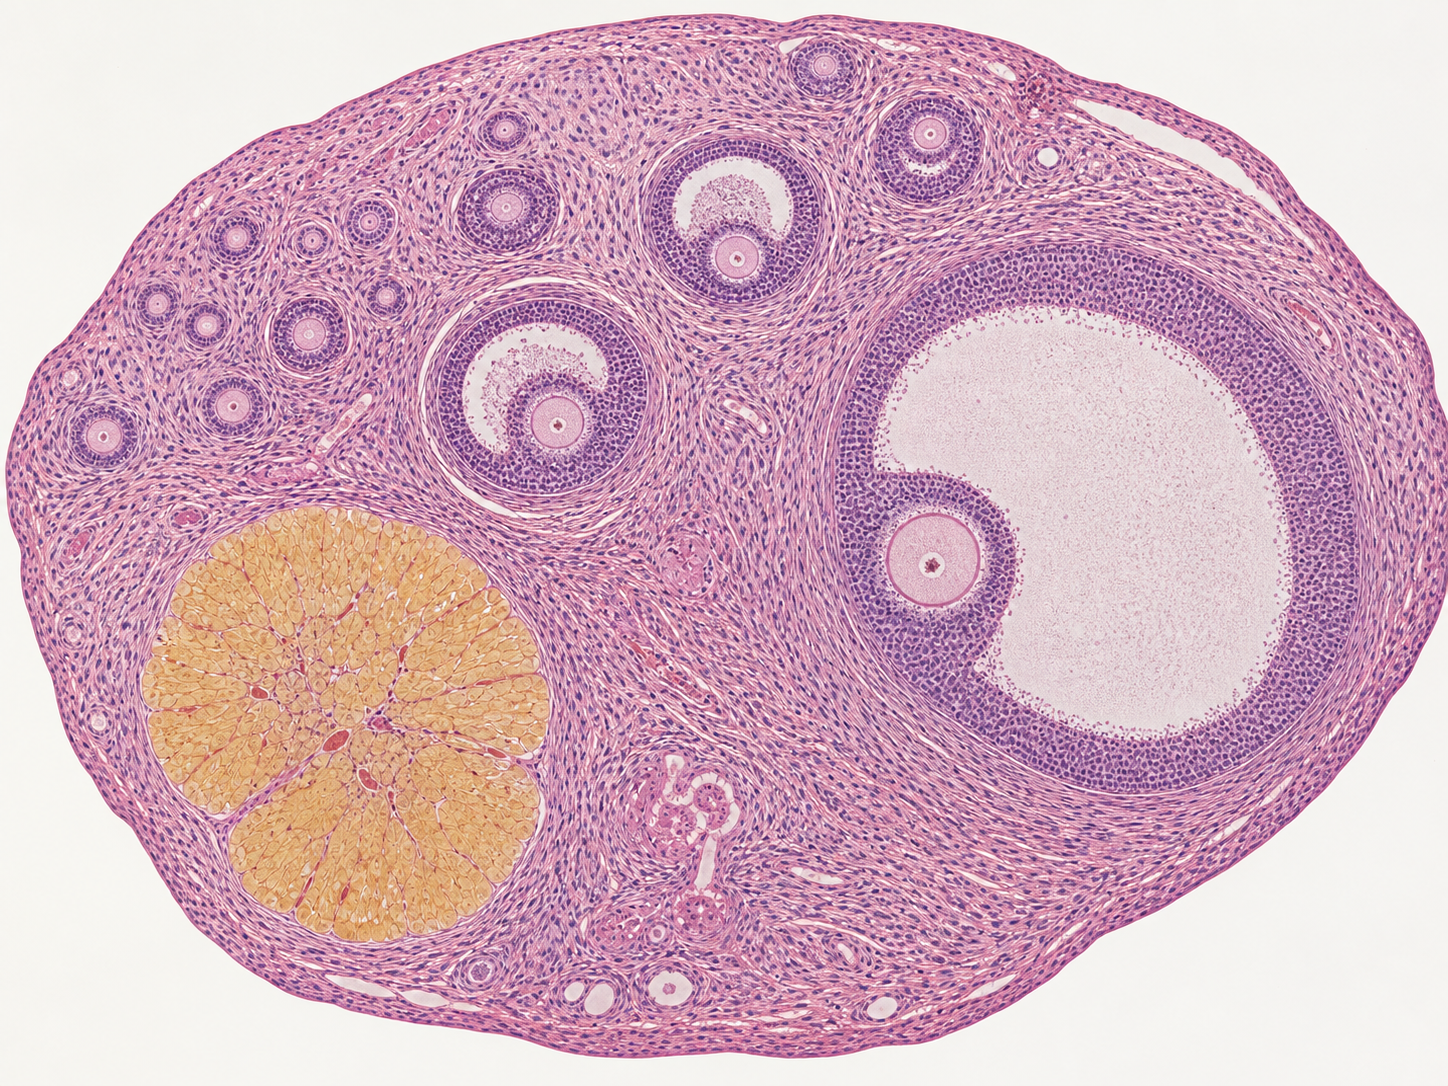
\includegraphics[width=0.56\linewidth]{images/book2/ai/g11-ovary-section.png}

{\small Een doorsnede van een eierstok: follikels in opeenvolgende
groeistadia, de grootste met haar met vocht gevulde holte en de eicel
erin, en een geel lichaam --- het overblijfsel van een follikel die een
eisprong heeft gehad.}
\end{omfigure}

\begin{proposition}[De baarmoedercyclus en de terugkoppelingen]\label{prop:g11:hormones-and-reproduction:uterus}
Het baarmoederslijmvlies volgt de \omterm{def:g11:hormones-and-reproduction:hormone}{hormonen} van de eierstok: oestrogenen
laten het tijdens de follikelfase dikker worden; progesteron maakt het
tijdens de gelefase afscheidend en klaar om een embryo te ontvangen; het
dalen van beide aan het eind van de cyclus laat het afbreken en bloeden
--- de \emph{menstruatie}, dag 1 tot 5 van de volgende cyclus. De
\omterm{def:g11:hormones-and-reproduction:hormone}{terugkoppelingen} wisselen tijdens de cyclus van teken: bij lage en matige
niveaus remmen oestrogenen en progesteron de hypothalamus en de hypofyse
(negatieve \omterm{def:g11:hormones-and-reproduction:hormone}{terugkoppeling}); maar het hoge oestrogeen van de rijpe
follikel, twee dagen volgehouden, \emph{prikkelt} hen (positieve
\omterm{def:g11:hormones-and-reproduction:hormone}{terugkoppeling}), en dat brengt de LH-uitschieter voort die de eisprong in
gang zet. Na de eisprong herstelt het progesteron van het gele lichaam de
negatieve \omterm{def:g11:hormones-and-reproduction:hormone}{terugkoppeling}, en volgt er geen tweede uitschieter.
\end{proposition}
\begin{proof}[Bewijsmateriaal]
Dagelijkse bloedmetingen leveren de krommen van de volgende figuur: de
LH-uitschieter volgt de oestrogeenpiek een dag later en gaat de eisprong
een dag vooraf; progesteron verschijnt pas na de eisprong. De eierstokken
verwijderen verhoogt LH en FSH; kleine doses oestrogenen verlagen ze; een
grote, volgehouden dosis halverwege de cyclus lokt een LH-uitschieter uit
--- het teken van de \omterm{def:g11:hormones-and-reproduction:hormone}{terugkoppeling} keert met de dosis om. Een vrouw
wier hypofyse niet op de oestrogeenstijging kan reageren, heeft geen
uitschieter en geen eisprong, hoewel haar follikels groeien.
\end{proof}

\begin{omfigure}
\begin{tikzpicture}
\begin{axis}[
  width=0.92\linewidth, height=6.4cm,
  axis x line=bottom, axis y line=left,
  xmin=0, xmax=28, ymin=0, ymax=122,
  xlabel={dag van de cyclus}, ylabel={hormoon (\% van zijn maximum)},
  xlabel style={font=\small, at={(axis description cs:0.5,-0.1)}, anchor=north},
  ylabel style={font=\small},
  tick label style={font=\small}, xtick={0,7,14,21,28}, ytick={0,50,100},
  legend style={at={(0.5,-0.22)}, anchor=north, legend columns=4, font=\small, draw=none},
  clip=false,
]
\addplot[thick, omMeth, smooth] coordinates {(0,10) (4,15) (8,30) (11,70) (12,100) (13,80) (14,45) (16,35) (19,55) (22,60) (25,40) (28,10)};
\addplot[thick, omProp, smooth] coordinates {(0,3) (12,3) (14,5) (16,30) (19,70) (21,100) (23,90) (25,55) (27,15) (28,5)};
\addplot[thick, omThm] coordinates {(0,15) (11,18) (12,35) (13,100) (14,60) (15,15) (28,12)};
\addplot[thick, omDef, dashed] coordinates {(0,45) (4,40) (9,30) (12,35) (13,70) (14,45) (15,20) (28,25)};
\draw[dashed, gray] (axis cs:14,0) -- (axis cs:14,113);
\node[font=\small, anchor=south] at (axis cs:14,113) {eisprong};
\draw[<->, gray] (axis cs:0.3,104) -- (axis cs:13.7,104);
\node[font=\scriptsize, anchor=south] at (axis cs:7,105) {follikelfase};
\draw[<->, gray] (axis cs:14.3,104) -- (axis cs:27.7,104);
\node[font=\scriptsize, anchor=south] at (axis cs:21,105) {gelefase};
\legend{oestrogenen, progesteron, LH, FSH}
\end{axis}
\end{tikzpicture}

{\small De \omterm{def:g11:hormones-and-reproduction:hormone}{hormonen} van één cyclus. De oestrogenen stijgen met de
groeiende follikel en pieken op dag 12; de LH-uitschieter volgt op dag 13
en de eisprong op dag 14; het progesteron, uit het gele lichaam,
overheerst de tweede helft en daalt aan het eind, wat de menstruatie
brengt.}
\end{omfigure}

\begin{omfigure}
\begin{tikzpicture}[font=\small, >=Stealth,
  b/.style={draw, rounded corners, align=center, text width=2.8cm, minimum height=1.0cm}]
  \node[b, fill=omDef!12] (h) at (0,3.2) {hypothalamus};
  \node[b, fill=omDef!12] (p) at (0,1.6) {hypofyse};
  \node[b, fill=omProp!15] (o) at (0,0) {eierstok};
  \node[b, fill=omMeth!15, text width=3.4cm] (u) at (6.4,0) {baarmoederslijmvlies:\\ wordt dikker, daarna\\ klaar voor een embryo};
  \draw[->, thick] (h) -- node[right] {GnRH} (p);
  \draw[->, thick] (p) -- node[right] {FSH, LH} (o);
  \draw[->, thick] (o) -- node[above, align=center] {oestrogenen,\\ progesteron} (u);
  \draw[->, thick, omThm, rounded corners=4pt] (o.west) -- (-2.3,0) -- (-2.3,3.2) -- (h.west);
  \node[omThm, anchor=east, align=right, text width=2.6cm] at (-2.45,0.9) {lage of matige niveaus remmen $(-)$};
  \draw[->, thick, omThm] (-2.3,1.6) -- (p.west);
  \draw[->, thick, omMeth!70!black] (o.north west) .. controls (-2.0,0.9) and (-2.0,2.3) .. (h.south west);
  \node[omMeth!70!black, font=\scriptsize, anchor=east, align=right, text width=2.4cm] at (-2.45,2.7) {hoog oestrogeen gedurende twee dagen prikkelt $(+)$: LH-uitschieter};
\end{tikzpicture}

{\small Regeling van de eierstok. Dezelfde keten als bij de man, met een
\omterm{def:g11:hormones-and-reproduction:hormone}{terugkoppeling} die van teken wisselt: negatief het grootste deel van de
maand, positief gedurende de twee dagen met de oestrogeenpiek die de
LH-uitschieter en de eisprong in gang zetten.}
\end{omfigure}

\begin{method}[Een cyclusschema lezen]\label{met:g11:hormones-and-reproduction:read}
\begin{enumerate}
  \item Zoek de LH-piek: de eisprong volgt de dag erna; de follikelfase
        is alles ervóór, de gelefase alles erna.
  \item Toets de volgorde: oestrogeenpiek, dan LH-uitschieter, dan
        eisprong, dan progesteron. Een kromme die uit de pas loopt, wijst
        op een stoornis.
  \item Tel: de gelefase duurt bij elke vrouw dicht bij 14 dagen; de
        lengte van de cyclus varieert in de follikelfase. De eisprong
        valt dus 14 dagen vóór de volgende menstruatie, en niet 14 dagen
        na de vorige.
  \item Leg een geneesmiddel of een beschadiging uit door je af te vragen
        welk \omterm{def:g11:hormones-and-reproduction:hormone}{hormoon} het toevoegt of wegneemt, en wat de \omterm{def:g11:hormones-and-reproduction:hormone}{terugkoppeling}
        dan met de andere doet.
\end{enumerate}
\end{method}

\section{Kiezen: anticonceptie}

\begin{proposition}[Hormonale anticonceptie]\label{prop:g11:hormones-and-reproduction:contraception}
De combinatiepil levert elke dag kleine doses van een oestrogeen en van
een progesteronachtig molecuul. Bij die niveaus is de \omterm{def:g11:hormones-and-reproduction:hormone}{terugkoppeling} de
hele tijd negatief: FSH blijft laag, geen enkele follikel rijpt, er komt
geen oestrogeenpiek, geen LH-uitschieter en geen eisprong. Het
baarmoederslijmvlies, dat dun wordt gehouden, en het slijm van de
baarmoederhals, dat dik wordt gehouden, voegen twee barrières toe. Een
week met de pillen stoppen laat de \omterm{def:g11:hormones-and-reproduction:hormone}{hormonen} dalen en het slijmvlies
bloeden. Andere methoden werken elders: een koperspiraaltje in de
baarmoeder voorkomt bevruchting en innesteling; de morning-afterpil,
binnen enkele dagen na de gemeenschap ingenomen, stelt de eisprong uit;
condooms verhinderen dat de gameten elkaar ontmoeten --- en zijn de enige
methode die ook seksueel overdraagbare infecties tegenhoudt.
\end{proposition}
\admitted

\begin{example}[Het effect van de pil aflezen]\label{ex:g11:hormones-and-reproduction:pill}
Op het schema van een vrouw die de pil gebruikt, lopen de vier krommen
vlak: oestrogenen en progesteron op het lage, gelijkmatige niveau dat de
pillen leveren, LH en FSH onder hun laagste waarde in de cyclus, en
nergens een piek. Wordt de pil vroeg in de strip enkele dagen vergeten,
dan ontsnapt FSH: er kan een follikel op gang komen, en de rest kan
volgen. De pil werkt omdat de \omterm{def:g11:hormones-and-reproduction:hormone}{terugkoppeling} werkt, en een vergeten pil
is een gat in de \omterm{def:g11:hormones-and-reproduction:hormone}{terugkoppeling}.
\end{example}

\section{Verkrijgen: geholpen voortplanting}

\begin{proposition}[Wanneer een zwangerschap uitblijft]\label{prop:g11:hormones-and-reproduction:art}
Ongeveer één paar op zeven zoekt na een jaar proberen hulp. De oorzaken
zijn over beide partners verdeeld: een uitblijvende of onregelmatige
eisprong, verstopte eileiders, te weinig of te weinig beweeglijke
zaadcellen, en in een derde van de gevallen geen aanwijsbare oorzaak. De
behandelingen volgen de biologie:
\begin{itemize}
  \item \emph{eisprong opwekken}: injecties met FSH, of een middel dat de
        negatieve \omterm{def:g11:hormones-and-reproduction:hormone}{terugkoppeling} van oestrogeen blokkeert, laten
        follikels rijpen; een injectie met een LH-achtige stof zet de
        eisprong daarna op een gekozen uur in gang;
  \item \emph{inseminatie}: bewerkte zaadcellen worden bij de eisprong in
        de baarmoeder gebracht;
  \item \emph{reageerbuisbevruchting}: na stimulatie worden eicellen met
        een naald uit de eierstok gehaald, in een schaaltje bevrucht ---
        zo nodig door in elke eicel één zaadcel te spuiten --- en worden
        drie tot vijf dagen later één of twee embryo's in de baarmoeder
        geplaatst. Ongeveer één poging op drie of vier leidt tot een
        geboorte; de rest kan met ingevroren embryo's worden herhaald.
\end{itemize}
Elke stap van de natuurlijke keten die faalt, wordt door de bijbehorende
ingreep vervangen.
\end{proposition}
\admitted

\begin{example}[De cijfers van één poging]\label{ex:g11:hormones-and-reproduction:ivf}
De stimulatie levert 10 eicellen op; 8 zijn rijp; 5 worden bevrucht; 3
bereiken het stadium van vijf dagen; 1 wordt teruggeplaatst en 2 worden
ingevroren. De terugplaatsing slaagt in ongeveer een derde van de
gevallen; met de twee ingevroren embryo's stijgt de kans op een geboorte
uit die ene oogst naar ongeveer 60\%. De techniek heeft sinds 1978 enkele
miljoenen kinderen voortgebracht; zij heeft ook vragen opgeroepen ---
over embryo's die niet worden gebruikt, over de leeftijd van ouders, over
wat er gekozen mag worden --- die de biologie niet beantwoordt.
\end{example}

\begin{remark}[Twee stelsels die elkaar ontmoeten]\label{rem:g11:hormones-and-reproduction:brain}
De \omterm{def:g11:hormones-and-reproduction:hormone}{hormonen} van dit hoofdstuk sturen de geslachtsklieren en het lichaam
aan; zij sturen bij de mens niet het seksuele gedrag aan zoals bij veel
dieren, waar de paring aan de eierstokcyclus is gekoppeld. Menselijke
seksuele activiteit staat grotendeels los van de cyclus en hangt af van
de stelsels van verlangen, plezier en hechting in de hersenen ---
beloningscircuits die met andere drijfveren worden gedeeld --- en van de
voorgeschiedenis, de cultuur en de keuzes van de persoon. Voortplanting
en seksualiteit overlappen elkaar; zij zijn niet hetzelfde, en de \omterm{def:g11:hormones-and-reproduction:hormone}{hormonen}
beheersen alleen het eerste.
\end{remark}

\section{Oefeningen}

\begin{exercise}[$\star$]\label{exo:g11:hormones-and-reproduction:1}
Definieer \omterm{def:g11:hormones-and-reproduction:hormone}{hormoon} en \omterm{def:g11:hormones-and-reproduction:hormone}{terugkoppeling}, en onderscheid negatieve van
positieve \omterm{def:g11:hormones-and-reproduction:hormone}{terugkoppeling}.
\end{exercise}

\begin{exercise}[$\star$]\label{exo:g11:hormones-and-reproduction:2}
Noem de drie lagen van de keten die de geslachtsklieren aanstuurt en de
\omterm{def:g11:hormones-and-reproduction:hormone}{hormonen} die elk ervan afscheidt.
\end{exercise}

\begin{exercise}[$\star$]\label{exo:g11:hormones-and-reproduction:3}
Wat zijn de twee afdelingen van de teelbal en wat brengt elk voort?
\end{exercise}

\begin{exercise}[$\star$]\label{exo:g11:hormones-and-reproduction:4}
Noem de fasen van de eierstokcyclus met hun \omterm{def:g11:hormones-and-reproduction:hormone}{hormonen}.
\end{exercise}

\begin{exercise}[$\star$]\label{exo:g11:hormones-and-reproduction:5}
Wat veroorzaakt de menstruatie?
\end{exercise}

\begin{exercise}[$\star\star$]\label{exo:g11:hormones-and-reproduction:6}
Geef uit de cyclusfiguur de dag van de oestrogeenpiek, van de LH-piek,
van de eisprong en van de progesteronpiek.
\end{exercise}

\begin{exercise}[$\star\star$]\label{exo:g11:hormones-and-reproduction:7}
Leg uit waarom castratie het LH verhoogt, en waarom een injectie
testosteron het weer verlaagt.
\end{exercise}

\begin{exercise}[$\star\star$]\label{exo:g11:hormones-and-reproduction:8}
Leg uit waarom de oestrogeenpiek van dag 12 een LH-uitschieter
voortbrengt, terwijl het oestrogeen van dag 20 dat niet doet.
\end{exercise}

\begin{exercise}[$\star\star$]\label{exo:g11:hormones-and-reproduction:9}
Een vrouw heeft cycli van 35 dagen. Op welke dag heeft zij haar eisprong?
Verantwoord dat.
\end{exercise}

\begin{exercise}[$\star\star$]\label{exo:g11:hormones-and-reproduction:10}
Leg uit hoe de combinatiepil de eisprong voorkomt, aan de hand van het
teken van de \omterm{def:g11:hormones-and-reproduction:hormone}{terugkoppeling}.
\end{exercise}

\begin{exercise}[$\star\star$]\label{exo:g11:hormones-and-reproduction:11}
Bij een man die testosteron gebruikt om te bodybuilden, krimpen de
teelballen en daalt het aantal zaadcellen. Verklaar dat.
\end{exercise}

\begin{exercise}[$\star\star\star$]\label{exo:g11:hormones-and-reproduction:12}
Een geneesmiddel blokkeert de oestrogeenreceptoren van de hypothalamus.
Voorspel het effect ervan op FSH, op de groei van follikels en op de
eisprong, en zeg waarom het bij sommige vormen van onvruchtbaarheid wordt
gebruikt.
\end{exercise}

\begin{exercise}[$\star\star\star$]\label{exo:g11:hormones-and-reproduction:13}
Het schema van een vrouw toont een oestrogeenpiek maar geen
LH-uitschieter en geen progesteron. Bepaal waar het gebrek in de keten
zit en stel een behandeling voor.
\end{exercise}

\begin{exercise}[$\star\star\star$]\label{exo:g11:hormones-and-reproduction:14}
Tijdens de zwangerschap scheiden de weefsels van het embryo een
LH-achtig \omterm{def:g11:hormones-and-reproduction:hormone}{hormoon} af dat het gele lichaam in leven houdt. Leg uit waarom
dat de menstruatie en verdere eisprongen voorkomt, en waarom
zwangerschapstests dat \omterm{def:g11:hormones-and-reproduction:hormone}{hormoon} opsporen.
\end{exercise}

\begin{exercise}[$\star\star\star$]\label{exo:g11:hormones-and-reproduction:15}
Bij een ivf-cyclus worden 12 eicellen geoogst, waarvan 60\% wordt
bevrucht en 40\% daarvan dag 5 haalt; elk teruggeplaatst embryo geeft in
35\% van de gevallen een geboorte. Bereken het verwachte aantal embryo's,
en de kans op ten minste één geboorte als zij één voor één worden
teruggeplaatst tot er een geboorte volgt of ze op zijn.
\end{exercise}

\section{Probleem: Het schema}

\begin{problem}[{Weekendprobleem --- de cyclus van één vrouw hormoon voor
hormoon in kaart gebracht, gelezen op haar terugkoppelingen, verstoord
door een pil, en geholpen wanneer zij faalt}]
\label{pb:g11:hormones-and-reproduction:1}
Er worden gedurende één cyclus dagelijks bloedmonsters genomen. Afgeronde
waarden, als percentage van het maximum van elk \omterm{def:g11:hormones-and-reproduction:hormone}{hormoon}:

\begin{center}
\begin{tabular}{lccccccccc}
dag & 2 & 6 & 10 & 12 & 13 & 14 & 18 & 22 & 27 \\ \hline
oestrogenen & 10 & 20 & 55 & 100 & 80 & 45 & 45 & 60 & 15 \\
LH & 15 & 15 & 20 & 35 & 100 & 60 & 15 & 15 & 12 \\
FSH & 45 & 35 & 30 & 35 & 70 & 45 & 22 & 25 & 25 \\
progesteron & 3 & 3 & 3 & 3 & 4 & 5 & 55 & 100 & 15 \\
\end{tabular}
\end{center}

\medskip
\noindent\textbf{Deel I --- Het schema lezen.}
\begin{enumerate}
  \item Op welke dag vindt de eisprong plaats? Verantwoord dat met twee
        \omterm{def:g11:hormones-and-reproduction:hormone}{hormonen}.
  \item Geef de follikelfase en de gelefase, met hun lengtes.
  \item Welke structuur van de eierstok scheidt de oestrogenen van dag 10
        af? En die van dag 22? Welke scheidt het progesteron van dag 22
        af?
  \item Beschrijf de toestand van het baarmoederslijmvlies op dag 6, 22
        en 28.
  \item Waarom is FSH aan het begin van de cyclus het hoogst en in de
        gelefase het laagst?
\end{enumerate}

\medskip
\noindent\textbf{Deel II --- De \omterm{def:g11:hormones-and-reproduction:hormone}{terugkoppelingen}.}
\begin{enumerate}[resume]
  \item Tussen dag 2 en dag 10 stijgen de oestrogenen terwijl FSH daalt.
        Welke \omterm{def:g11:hormones-and-reproduction:hormone}{terugkoppeling} is aan het werk? Leg dat uit.
  \item Tussen dag 12 en dag 13 staan de oestrogenen op hun piek en
        stijgt LH zevenvoudig. Welke \omterm{def:g11:hormones-and-reproduction:hormone}{terugkoppeling}? Welke voorwaarde
        aan het oestrogeenniveau maakt dat mogelijk?
  \item Tussen dag 18 en dag 27 zijn de oestrogenen matig, is het
        progesteron hoog en is LH laag. Welke \omterm{def:g11:hormones-and-reproduction:hormone}{terugkoppeling}, en waarom
        volgt er geen tweede uitschieter?
  \item Het gele lichaam takelt op dag 26 af. Voorspel de \omterm{def:g11:hormones-and-reproduction:hormone}{hormonen} van
        dag 28 en wat daarop volgt.
  \item Leg uit waarom de cyclus zichzelf opnieuw start: welke stijging
        op dag 1 zet de volgende follikel op gang?
\end{enumerate}

\medskip
\noindent\textbf{Deel III --- De pil.}
Dezelfde vrouw gebruikt een maand lang de combinatiepil, die elke dag
oestrogenen op 25\% en een progesteronachtig \omterm{def:g11:hormones-and-reproduction:hormone}{hormoon} op 40\% van hun
maxima levert.
\begin{enumerate}[resume]
  \item Voorspel de niveaus van FSH en LH gedurende de hele maand, en het
        lot van de follikels.
  \item Komt er een oestrogeenpiek? Een LH-uitschieter? Een eisprong?
  \item Wat gebeurt er tijdens de zeven pilvrije dagen met het
        baarmoederslijmvlies, en waarom is dat geen echte menstruatie?
  \item Zij vergeet de pillen op dag 5 tot en met 8. Leg het risico stap
        voor stap uit.
  \item Leg uit waarom ook een pil met alleen progesteron, op een niveau
        dat de negatieve \omterm{def:g11:hormones-and-reproduction:hormone}{terugkoppeling} in stand houdt, de eisprong kan
        voorkomen.
\end{enumerate}

\medskip
\noindent\textbf{Deel IV --- Wanneer de keten faalt.}
\begin{enumerate}[resume]
  \item Het schema van een andere vrouw toont FSH en LH steeds onder 10\%
        en oestrogenen onder 10\%. Waar zit het gebrek? Welke behandeling
        zou de eisprong herstellen, en langs welke weg?
  \item Het schema van een derde vrouw is normaal, maar haar eileiders
        zijn verstopt. Welke stappen van
        \cref{prop:g11:hormones-and-reproduction:art} vervangen de
        geblokkeerde stap?
  \item Bij ivf wordt 36 uur vóór het oogsten van de eicellen één injectie
        met een LH-achtig \omterm{def:g11:hormones-and-reproduction:hormone}{hormoon} gegeven. Leg uit wat die nabootst en
        waarom de timing precies moet zijn.
  \item Na de stimulatie rijpen er 10 follikels in plaats van 1. Leg met
        FSH uit waarom de natuurlijke cyclus er meestal maar één laat
        rijpen.
  \item Geef het resultaat: de dag van de eisprong op het schema, de twee
        tekenen van de \omterm{def:g11:hormones-and-reproduction:hormone}{terugkoppeling} die haar voortbrachten, en het
        mechanisme waarmee de pil haar onderdrukte.
\end{enumerate}
\end{problem}
